\documentclass[a4paper,ngerman, 14pt] {scrartcl}
\usepackage[T1]{fontenc}
\usepackage[utf8]{inputenc}
\usepackage[ngerman]{babel}
\usepackage{blindtext}
\usepackage{csquotes}
\usepackage{hyperref}
\usepackage{graphicx}
\usepackage{caption}
\usepackage{setspace}
\usepackage{MnSymbol}
\usepackage[top=2cm, bottom=3.5cm, left=3cm, right=2.5cm]{geometry} 

\begin{document}
\tableofcontents
\newpage
\section{Einleitung}
Der AsTA hat vor einiger Zeit den Entschluss gefasst, ein Pedelec Lastenrad zu erwerben, um es als Leihrad für die Studierenden anzubieten. Es soll das mittlerweile mittlerweile nicht mehr fahrtüchtige Lastenrad im Bestand ersetzen. Ziel ist im Bereich Lastentransport den Studierenden Alternativen zum Auto zu bieten und nachhaltige Mobilität zu fördern.\\
Zu diesem Zweck ist Erik Wohlfeil, Nachhaltigkeitsbeauftragter des Studierendenparlaments an uns, den Arbeitskreis Fahrradcampus, herangetreten mit der Bitte um technische Unterstützung bei der Anschaffungsentscheidung. Eine frühere Kaufempfehlung existierte bereits, Diese kann aber angesichts der mittlerweile geänderten Marktlage als nichtig erachtet werden.\\


\section{Anforderungen die das Rad stellt}
Ein hochwertiges modernes Fahrrad stellt andere Anforderungen an die Nutzer:innen, als man es vielleicht von älteren Rädern gewohnt ist. Längerfristige Nutzung eines Lastenpedelecs stellt folgende Anforderungen:\\

\subsection{Regelmäßige Wartung bei einer Fachwerkstatt.} Am besten ist es eine feste Vereinbarung mit einem Fachhändler einzugehen, idealerweise der Selbe bei dem das Rad erworben wurde.

\subsection{Schutz vor Witterung.} Ein Rad und ein Pedelec im Besonderen dürfen bei Nichtnutzung nicht einfach im Freien stehen, wie es mit dem alten Lastenrad Usus war. Eine Unterstellmöglichkeit muss daher vorhanden sein. Schutz vor Witterung ist das Wichtigste, Schutz vor Kälte ist erstrebenswert, aber nicht zwingend notwendig.

\subsection{Kurze Unterrichtung von Neunutzer:innen.} Die Technik eines Pedelecs und das andere Fahrverhalten eines Lastenrad erfordern das Nutzer:innen die nicht mit diesen Dingen vertraut sind eine kurze Einweisung erhalten. Jede Person, die den Lastenradverleih durchführt, sollte diese kurze Einweisung geben können und ggfs. eine kurze Anpassung an Nutzer:innen durchführen.\\
\vspace{2mm}\\
\textit{All diese Punkte müssen vor der Anschaffung geklärt sein.}


\section{Grundvorraussetzungen an das Rad}
Bevor wir in die engere Auswahl gegangen sind haben wir einen Grundrahmen formuliert in den alle Räder passen müssen. Folgende Punkte kamen zusammen:\\
\subsection{Long John Rahmenform.} Lastenräder gibt es in vielen unterschiedlichen Konfigurationen. Von Anfang an war klar, dass nur Zweiräder in Frage kommen, da sich Dreirädern bei Kurvenfahrten unvorhersehbar verhalten. Die Long-John-Konfiguration, bei der die Ladefläche tief vor dem Lenker liegt, ermöglicht es die Länge des Rades verlässlich während der Fahrt einzuschätzen und liefert durch den tiefen Schwerpunkt ein sicheres Fahrverhalten.

\subsection{Mittelmotor.} Die Motorisierung eines Fahrrads kann an drei Punkten erfolgen: in der Vorderradnabe, an der Kurbel oder in der Hinterradnabe. Frontmotoren liefern in unseren Augen kein zufriedenstellendes Unterstützungsverhalten. Heckmotoren tun dies, jedoch neigen sie in der Hand von weniger erfahrenen Nutzer:innen zum Überhitzen unter Last. Mittelmotoren haben den größten Marktanteil unter den Pedelecs, sie liefern verlässliche und kontrollierbare Unterstützung, und haben den derzeit höchsten technischen Reifegrad unter den Antriebssystemen.

\subsection{Hydraulische Scheibenbremsen.} Hohes Gewicht des Fahrrads und elektrische Unterstützung erfordern angemessene Bremsen. Manche Hersteller setzen an diesem Punkt leider manchmal den Rotstift an. Hydraulische Scheibenbremsen sind unserer Meinung nach das Mindeste, idealerweise mit großen Bremsscheiben oder sogar vier Bremskolben statt der üblichen zwei.

\subsection{Nabenschaltung.} Das Lastenrad wird in den Händen der Studierenden \textbf{nicht zimperlich} behandelt werden. Wichtig ist daher intuitive Bedienbarkeit und Robustheit gegenüber Fehlbedienung. Boshaft formuliert: Es muss idiotensicher sein. In diesem Anwendungsfall bieten sich gekapselte Nabenschaltungen gegenüber einer Kettenschaltung an, hier gibt es keine exponierten Teile und das Risiko einer Beschädigung durch Missbrauch ist deutlich geringer.
\subsection{Anpassbarkeit.} Lastenräder kommen nahezu ohne Ausnahme in genau einer Größe. Aus diesem Grund treffen die meisten Hersteller Maßnahmen, um das Rad einem möglichst großen Spektrum an Fahrer:innen nutzbar zu machen. Die Wirksamkeit dieser Maßnahmen variiert zwischen Modellen.
\newpage


\section{Tests}
Unerlässlich für eine Entscheidungsfindung sind Praxistests, diese fanden bis jetzt in zwei Formen statt. Einer der Autoren ist in einem Radladen tätig und hat dadurch Berührungspunkte mit Lastenrädern, weiterhin wurde der Halt der Cargobike Roadshow in Böblingen am 20.09.2020 genutzt, um weitere Räder zu testen.

\subsection{Bakfiets Classic Long Steps SS8.}
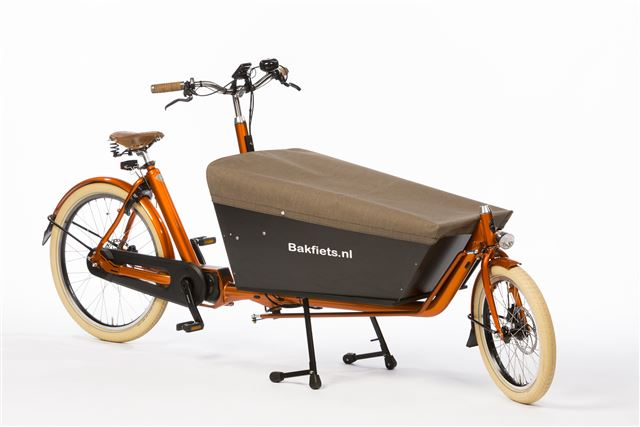
\includegraphics[scale=0.8]{bakfiets_long_steps.jpg}\\
Ein Bakfiets Modell wird in besagtem Radladen als Ausstellungsobjekt genutzt, sowie zum Transport von Kindern, Getränken und manchmal auch anderen Fahrrädern.\\
Das Bakfiets kann leider nicht auf ganzer Linie überzeugen. Die Fahrstabilität ist unterer Durchschnitt und Anpassbarkeit gut, in den Details fallen die Dinge jedoch auseinander. Im Hinblick auf Wartung ist das Rad eine Zumutung, Schwächen in Verarbeitung und Konstruktion trüben das Bild weiter. Die Bedienung der Parkstütze ist unnötig hakelig.\\ Mit 4030€ ist das Rad vergleichsweise preiswert.
\subsection{Ca Go FS 200.}

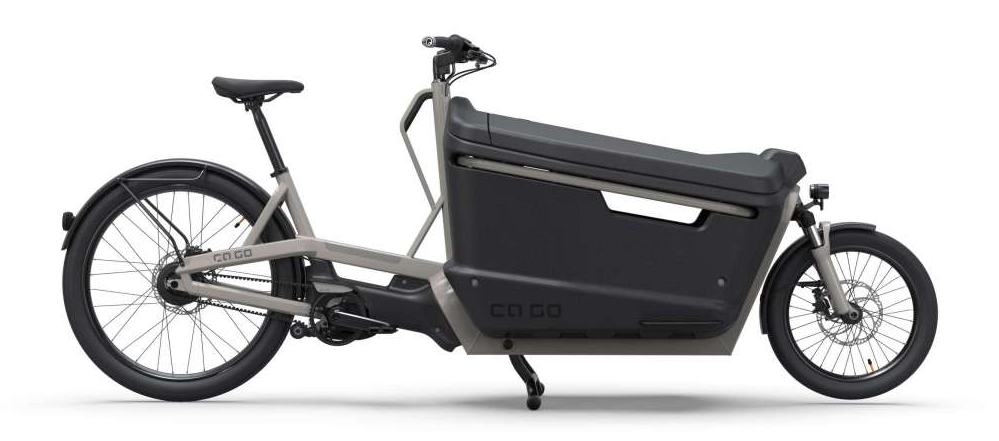
\includegraphics[scale=0.54]{ca_go.png}\\
Beim Testevent in Böblingen stach das Ca Go heraus. Eine brandneue Entwicklung, vollgestopft mit state-of-the-art Technik. Feinste Komponenten, integrierte Displays, hydraulisch unterstützter Deckel für die Ladebox und mehr.\\
Die Kehrseite des High-Tech ist dass wir es für ein wenig zu sensibel für den Verleih erachten. Weiterhin war die Lenkung schwammig, ein schwerlich akzeptabler Kompromiss für ca 6500€.

\subsection{Urban Arrow Family.}
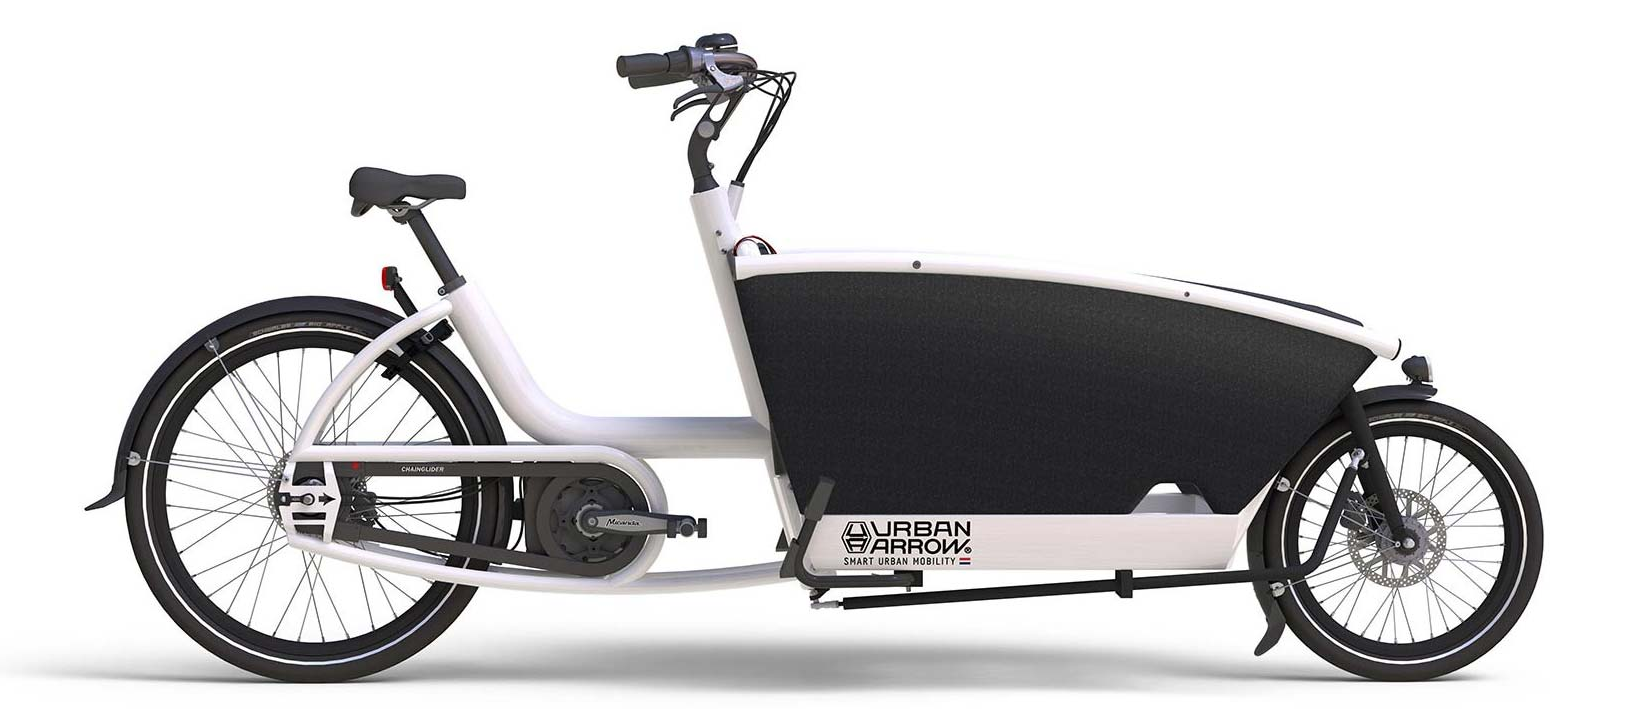
\includegraphics[scale=0.325]{urban_arrow_family.png}\\
Die Firma Urban Arrow hat sich auf E-Lastenräder spezialisiert, das Family stellt die goldene Mitte des Programms dar, flankiert vom deutlich kompakteren Shorty und dem größeren Cargo. Beim Namen denkt man eher an Kindertransport, jedoch ist das Family auch ein sehr ausgeglichener Lastenträger.\\
Die Fahreigenschaften sind der Trumpf, selbst völlige Neulinge beim Thema Lastenrad und E-Bike waren bereits nach wenigen Sekunden souverän auf dem Urban Arrow unterwegs. Ebenfalls ansprechend sind die bei der Ausstattung getroffenen Entscheidungen, eine starre Gabel verspricht Wartungsarmut, genauso die stufenlose Enviolo Schaltung. Die Konstruktion des Rahmens ist durchdacht.\\
Getestet wurde das Topmodell mit Bosch Cargo Line Motor und Shimano Zee Vierkolben-Bremsen, allerdings sollte das Modell darunter mit dem etwas schwächeren Active Line Motor und Zweikolben-Bremsen ausreichen. Anpassbarkeit an den Fahrer ist gut, die Konfiguration der Ladefläche ist allerdings nicht sehr flexibel.\\
Preislich bewegt sich das Rad im Mittelfeld mit 5000€ für die Active Line Version und 5400€ für die Cargo Line.\\
\textit{Aufgrund der hervorragenden Fahreigenschaften ist das Urban Arrow die definitive Empfehlung aus den getesteten Rädern. Kein Rad vermittelte beim Testen das selbe Maß an Fahrsicherheit wie das Family.}

\subsection{Urban Arrow Cargo.}
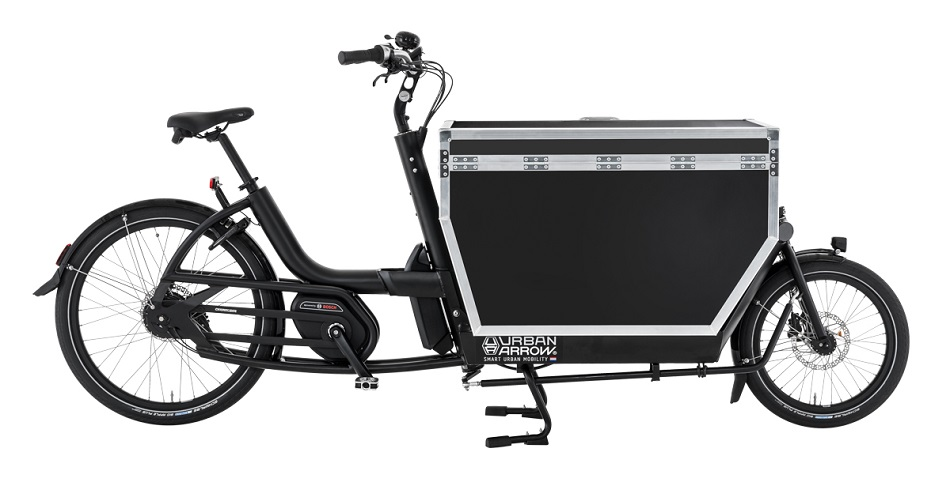
\includegraphics[scale=0.415]{urban_arrow_cargo.jpg}\\
Das Cargo ist das lastenorientierte Ende der Urban Arrow Produktpalette. Es besitzt eine längere und deutlich flexiblere Ladefläche als das Family, mit mehreren verfügbaren Aufbauten. Ebenfalls anders als beim Family ist eine Federgabel verbaut, in unseren Augen kein Vorteil da sie ein weiteres bewegliches Teil darstellt.\\
Im Vergleich fährt sich das Cargo etwas sperriger als das Family, auch die Fahrstabilität, wenngleich solide, reicht nicht ganz an die kompaktere Markenschwester heran.\\
Das günstigere Modell mit Shimano Deore Scheibenbremsen wird für 4100€ verkauft, weiterhin muss man nochmal ca 1000€ für den ausgewählten Ladeflächenaufbau einrechnen. Das Urban Arrow Cargo erhält eine eindeutige Empfehlung, wenn die Tragekapazitäten des Family als nicht ausreichend erachtet werden.

\subsection{Cube Cargo Hybrid.}
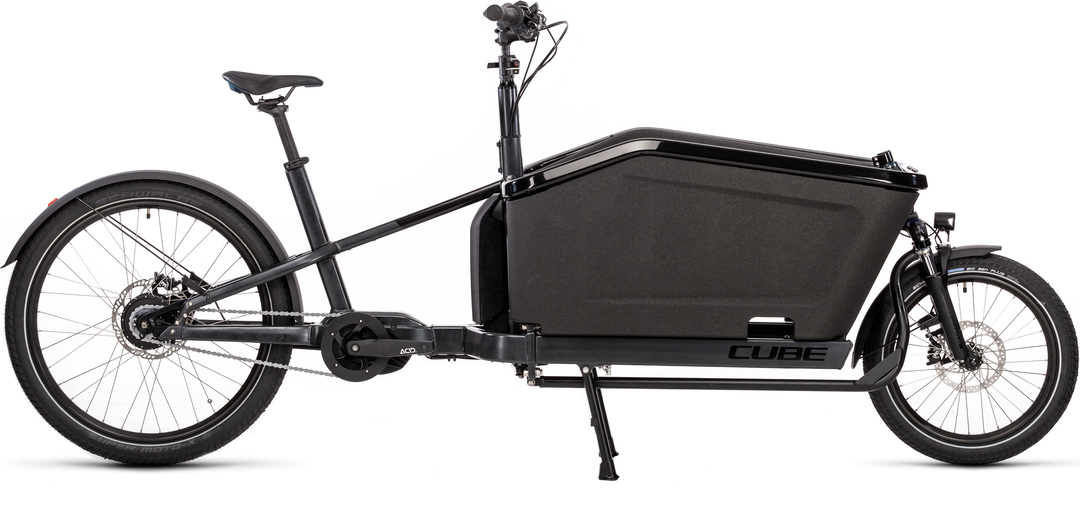
\includegraphics[scale=0.36]{cube_cargo_hybrid.jpg}\\
Mit Cube ist jetzt auch ein größerer Hersteller konventioneller Fahrräder auf den Lastenradzug aufgesprungen. Das Cargo Hybrid war in der \grqq{Sport} Variante mit Kettenschaltung als Testrad zugegen, ist allerdings Baugleich mit dem nicht-Sport Hybrid, das über die Enviolo Nabenschaltung verfügt und daher auch den Vorzug erhalten sollte.\\
In Sachen Fahrverhalten hält sich das Rad unauffällig im Mittelfeld, ohne an die Urban Arrows heranzukommen. Hervorzuheben ist die hervorragende Anpassbarkeit über den Speedlifter Vorbau und die kräftigen Vierkolben-Scheibenbremsen. Ein Upgrade auf das \grqq{Dual Hybrid} mit doppelten Akkupack ist nicht nötig in unseren Augen.\\
Das Cube kostet 4700€.

\subsection{Radkutsche Rapid.}
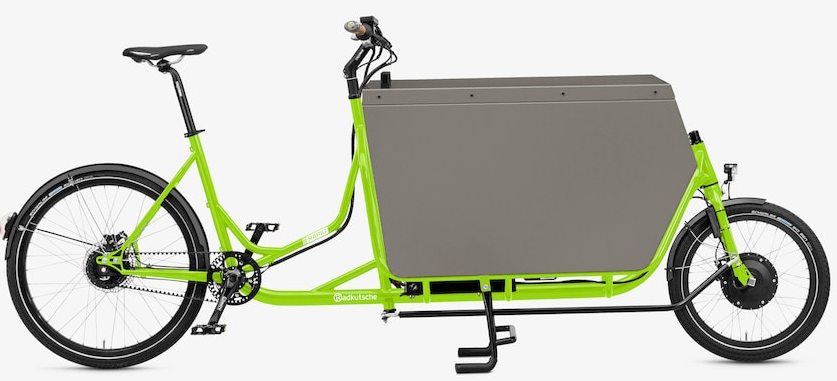
\includegraphics[scale=0.64]{radkutsche_rapid.png}\\
Radkutsche ist ein Anbieter aus dem Raum Stuttgart, war daher auch dementsprechend stark beim Testevent vertreten. Ab nächstem Jahr wird es auch Modelle mit Mittelmotor geben, Stand September 2020 gab es allerdings lediglich Frontmotoren zu testen. Die Rahmenkonstruktion soll jedoch weitestgehend gleich bleiben.\\
Radkutsche bietet einen umfangreichen Konfigurator sowie einen erfrischenden \grqq{keep it simple} Ansatz im Hinblick auf Technik, ohne die wichtigen Dinge aus dem Blick zu verlieren.\\
Leider können die Fahreigenschaften nicht mithalten. Der Rahmen ist zu filigran und braucht eine erfahrene Hand, um sicher bewegt zu werden. Die Problematik verschärft sich mit zunehmender Beladung nur weiter. Umfassende Anpassbarkeit an verschiedene Fahrer:innen ist auch nicht wirklich gegeben, die eigentliche Achillesferse ist und bleibt aber das Fahrverhalten, dadurch leider keine Empfehlung.\\
Ein fester Preis für die Mittelmotor-Version ist zur Zeit noch nicht abzusehen wird sich aber wahrscheinlich jenseits der 5000€ bewegen.
\newpage


\section{Zusammenfassung}
Die Zusammenfassung lässt sich knapp halten: Die Urban Arrow Modelle überzeugen im Fahrversuch am meisten. Die zusätzliche Kapazität des \grqq{Cargo} ist unserer Meinung nach nicht nötig.\\
Zweite Wahl wäre das Cube Cargo Hybrid.
\end{document}